\documentclass[10pt]{article}\usepackage[margin=.7in]{geometry}\usepackage{graphicx}\begin{document}\section*{Publication custody audit}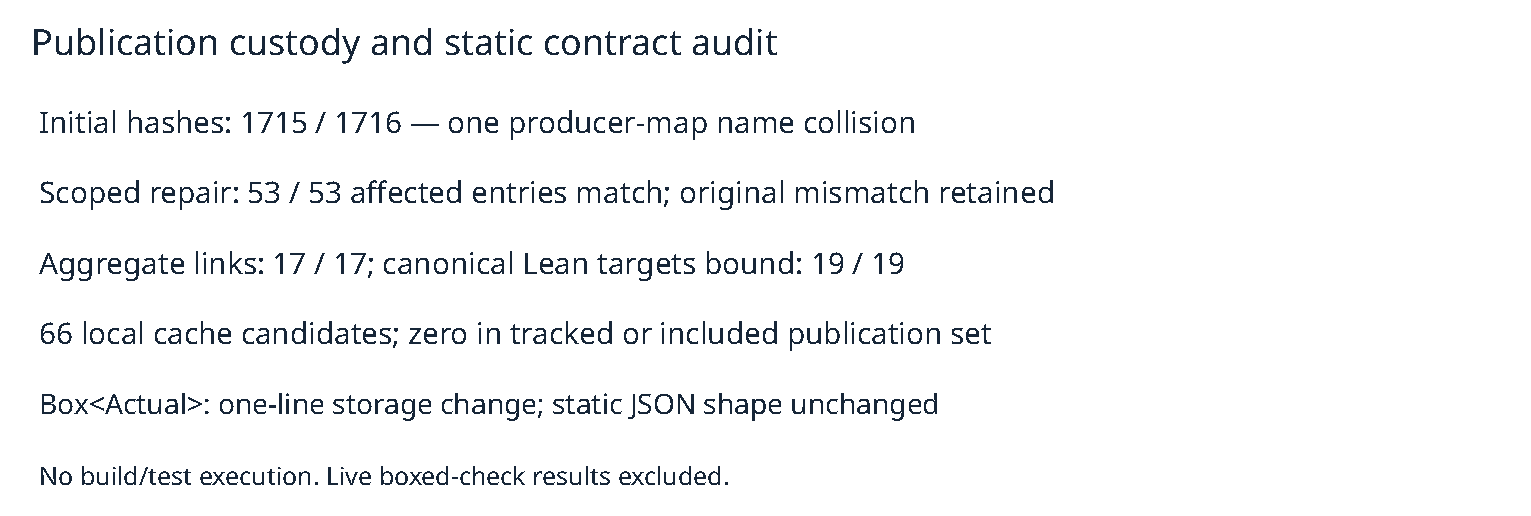
\includegraphics[width=\linewidth]{figure.pdf}
\paragraph{Custody repair} The initial pass found a producer custody-map copied under the same basename as its new publication map. Root restored the original under producer-custody-map.json and recorded the correction. All53 included entries in that affected map now match; the initial mismatch remains retained. Other initially matching entries were not rehashed after repair.

\paragraph{Canonical source bindings} All19 registered modules match retained snapshots. Constructor and Add11 use only the explicitly documented terminal-newline normalization; original reviewed bytes remain retained. This is source custody, not a new proof compilation.

\paragraph{Publication set} None of66 local compiled/render-cache candidates occurs in the1,957 narrowly enumerated tracked paths or is claimed included by a custody map. Local build caches remain present. Render source and log receipts are distinguished from compiled caches.

\paragraph{Static JSON contract} The exact change against da1464 is actual:Actual to actual:Box<Actual>. Resolved Serde forwards deserialization to Actual and wraps the result, preserving JSON fields, tags and rejection policy. Boxing changes storage/allocation. No dynamic validation is inferred; root's live boxed-request checks were excluded.

\paragraph{Artifacts} REVIEW.md preserves source analysis; status.json, custody-checks.json, canonical-bindings.json, aggregate-links.json and postrepair.json retain exact scope and receipts. No repository edits, builds, tests, cloud actions or scientific execution were performed by this audit.
\end{document}